% Source: figs/src/refpipeline.py (python3 figs/src/refpipeline.py writes
% figs/fig_refpipeline.pdf and .png).
\begin{figure*}[t]
\centering
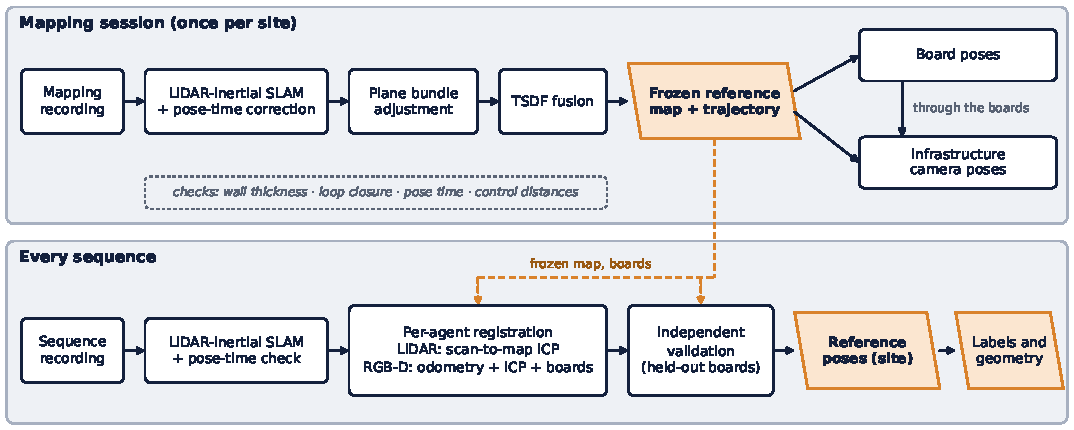
\includegraphics[width=\textwidth]{figs/fig_refpipeline.pdf}
\caption{Reference pipeline. Top: the mapping session, run once per site.
The SLAM trajectory, corrected for its pose-time offset, is refined by
plane bundle adjustment and the scans are fused into a TSDF map; map and
trajectory are then frozen, the boards are posed in them
(Eq.~\eqref{eq:board_chain}) and the infrastructure cameras placed
through the boards (Eq.~\eqref{eq:infra_camera_chain}). Wall thickness,
the board loop closure, the pose time and control distances check the
result. Bottom: each sequence is registered into the frozen map, by
scan-to-map ICP for the LiDAR agents and by odometry with ICP and board
factors for the RGB-D agent, validated on held-out boards, and exported
in the site frame.}
\label{fig:refpipeline}
\end{figure*}
